\documentclass[11pt,a4paper]{article}
\usepackage[T1]{fontenc}\usepackage[utf8]{inputenc}
\usepackage[margin=22mm]{geometry}\usepackage{amsmath,booktabs,graphicx,hyperref}
\title{Rogelio v3: input charge and the 14 mV signal}
\author{NAUSICA calculation record}\date{\today}
\begin{document}\maketitle
The supplied v3 pulse produces an output drop of 13.9074 mV. Its
integrated input charge is 0.0816001 fC, equivalent to 509.31 elementary
charges. The paper's 1000-ion current applied to exactly the same circuit
produces 27.2728 mV. The approximately 14 mV result is therefore consistent
with the paper: the supplied test injects about half as much charge.

\section*{Reproduction}
The circuit is read from
\texttt{LTSpice/Spice2/v3/CSAfolded180nm-2\_Astronio.asc}, with its supplied
model card. It uses the paper's transistor dimensions, 3 fF feedback,
1.25 pF external input capacitance and $20\,^{\circ}$C. Its gate voltages
are 0.53847 V for M3 and 0.556803 V for M4. The output baseline is
0.888809 V. The source is
\begin{center}\texttt{EXP(0 48f 200m 0.05n 0 1.7m)}.\end{center}
The simulated current begins at 0.2 s, reaches 48 fA and decays with a
fitted time constant of 1.7 ms. Its integral is consistent with
$48\,\mathrm{fA}\times1.7\,\mathrm{ms}=0.0816\,\mathrm{fC}$.
The schematic annotation ``0.5 ke = 0.8 fC'' has a factor-ten error;
500 elementary charges correspond to approximately 0.08 fC.

\begin{center}\begin{tabular}{lrrr}\toprule
Input & Charge (fC) & Charge ($e$) & Output drop (mV)\\\midrule
Supplied exponential & 0.0816001 & 509.31 & 13.9074\\
1000 ions, uniform over 20 ms & 0.1599633 & 998.41 & 27.2728\\\bottomrule
\end{tabular}\end{center}
The uniform-ion current retains the original finite-path normalization.
It uses the central 0.5 mm square pad in a grounded plane, homogeneous gas,
and a central 5 mm approach at 3 m/s. The weighting potential is one on
the pad, zero on the remaining plane and zero at infinity. Each ion
contributes $e\Delta\phi_w$ rather than being renormalized to $e$.

\begin{figure}[htbp]\centering
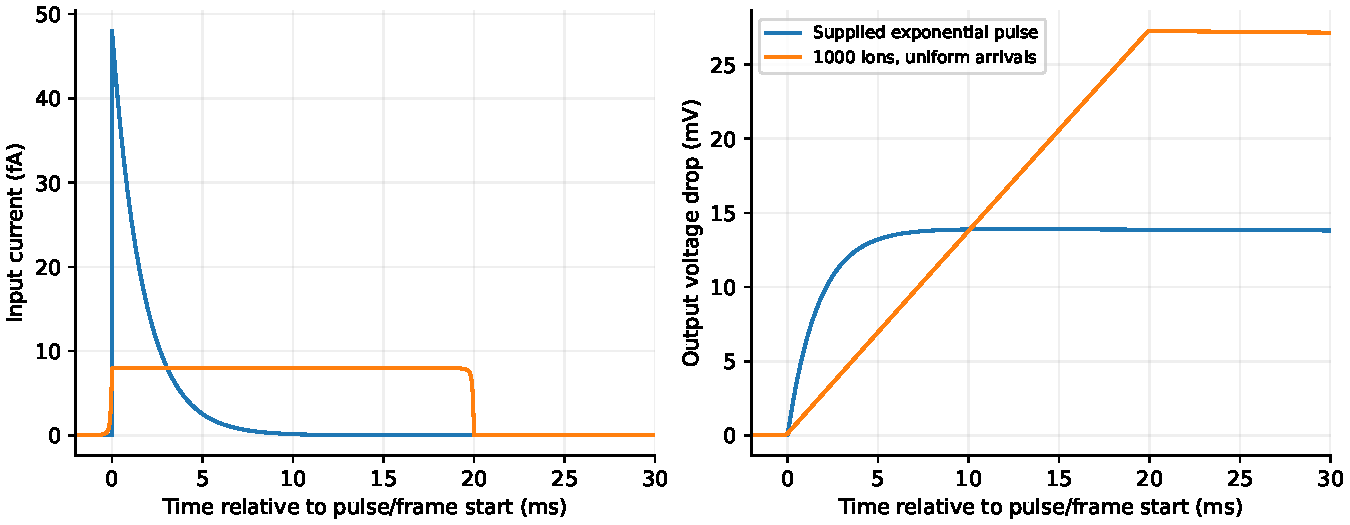
\includegraphics[width=\linewidth]{pulse_comparison.pdf}
\caption{Both input waveforms simulated with the supplied v3 circuit.}
\end{figure}

\section*{Charge integration and convergence}
The calculation uses maximum timesteps of 5 and 2.5 $\mu$s, tight solver
tolerances and disabled waveform compression. Integrating the saved input
current agrees with the independent behavioral \texttt{idt(I(Is1))}
accumulator. Step refinement changes the charge by 0.00020\% and the
output peak by 0.0013\%.
The original 40 s run reproduces the approximately 14 mV pulse, but its
compressed current trace is unsuitable for charge integration. The supplied
\texttt{.meas} result must be checked with resolved, uncompressed current data.

\section*{Resistance label}
The schematic's resistance label evaluates \texttt{V(out)/Id(M4)}. At this
operating point it gives -2.323 M$\Omega$. This is a DC ratio involving
the output node voltage. M4's incremental drain resistance is
$r_o=1/g_{ds}$, which the operating-point log gives as approximately
28.8 M$\Omega$. These are different quantities; the displayed ratio does
not establish the amplifier's small-signal voltage gain.

\section*{Reproduction commands}
Acquisition is \texttt{scripts/run\_rogelio\_v3.py}; Julia analysis is
\texttt{scripts/analyze\_rogelio\_v3.jl}; presentation is
\texttt{scripts/present\_rogelio\_v3.py}. Commands and saved data are in
\texttt{results/ltspice/rogelio\_v3/README.md}. The manuscript is unchanged.
\end{document}
